% ============================================================================
%  PRISM-4D v4.0 -- Publication-Ready Manuscript
%  For Springer Nature submission, replace sn-jnl.cls with official version
%  All remediation tasks from reframing ledger applied
%  All equations numbered, all acronyms defined, all claims qualified
% ============================================================================
\documentclass{sn-jnl}

% ---- Additional packages ----
\usepackage{amsmath,amssymb}
\usepackage{graphicx}
\usepackage{booktabs}
\usepackage{hyperref}
\usepackage{xcolor}
\usepackage{multirow}
\usepackage{caption}
\usepackage{float}
\usepackage{enumitem}

\hypersetup{
  colorlinks=true,
  linkcolor=snblue,
  citecolor=snblue,
  urlcolor=snteal
}

% ---- Custom colors for tables ----
\definecolor{excellent}{RGB}{46,139,87}
\definecolor{good}{RGB}{0,128,128}
\definecolor{marginal}{RGB}{204,153,0}
\definecolor{novelgold}{RGB}{184,134,11}

\title{\color{snblue}PRISM-4D: Spike-Event-Driven Detection of Cryptic
Binding Sites via Physics Simulation}
\author{Ididia Serfaty\\
{\small Delfictus IO LLC, \texttt{is@delfictus.com}}\\[2pt]
{\small\color{sngray} Preprint -- February 2026}}
\date{}

\begin{document}

\twocolumn[\maketitle
\begin{center}
\parbox{0.92\textwidth}{\small
\textbf{Abstract.}
\noindent\textbf{Background:}
Cryptic binding sites---transient pockets absent in static crystal structures---represent
high-value drug targets inaccessible to conventional computational screening. Existing
methods rely on surface geometry (fpocket, SiteMap) or machine learning trained on
crystallographic features (P2Rank, DeepSite), inherently limiting their capacity to detect
conformationally gated pockets.

\smallskip\noindent\textbf{Methods:}
We introduce PRISM-4D (Physics-driven Recognition of Intrinsic Sites through Molecular 4D
dynamics), a platform that detects cryptic binding sites through explicit physics simulation
rather than geometric inference or statistical learning. PRISM-4D couples AMBER ff14SB force
field molecular dynamics with a 5-phase cryo-thermal hysteresis protocol
(50\,K$\to$300\,K$\to$50\,K; 55{,}000 steps per stream), multi-wavelength UV excitation
spectroscopy simulation (280/274/258/254/211\,nm), and a leaky integrate-and-fire (LIF)
neuromorphic network to identify cooperative dewetting events indicative of druggable pocket
formation. Detected spike events are clustered via Spike-Native Density Clustering (SNDC), a
4-stage GPU pipeline comprising RT-DBSCAN via OptiX bounding volume hierarchy (BVH)
traversal, watershed segmentation, Eikonal BFS distance-field computation, and
intensity$^2$-weighted centroid tracking.

\smallskip\noindent\textbf{Results:}
On a 12-protein benchmark spanning orthosteric, allosteric, and cryptic binding sites,
PRISM-4D detects all 11 ground-truth targets within 10\,\AA{} Distance from Centroid to
Centroid (DCC), the Euclidean distance between predicted and crystallographic ligand centroids
after Kabsch superposition (range: 3.6--9.8\,\AA{}). Four targets (36.4\%) achieve $<$5\,\AA{}
and eight (72.7\%) achieve $<$8\,\AA{}. On the SIRP$\alpha$ immune checkpoint protein,
PRISM-4D detects the experimentally validated WYF cryptic pocket (7.1\,\AA{} DCC, top-ranked)
from the closed apo structure; P2Rank 2.5 assigns 0.2\% probability to the same pocket. On
$\beta$-catenin, PRISM-4D identifies a computationally predicted cryptic pocket (Site~6)
featuring a dual-cysteine pair (CYS240/CYS278) with quality 0.965 and centroid displacement
$<$0.06\,\AA{} across 5 stochastic seeds. In a post-freeze blind Vectorial Pharmacophore
Feature Recovery (PFR) audit, phase-ordered PRISM4D manifolds achieve 26.9\% Vectorial PFR
versus 2.2\% for a temporal-scramble null (12.2-fold enrichment; empirical $p \leq 0.001$),
demonstrating that nonequilibrium phase ordering is load-bearing for directional pharmacophore
recovery.

\smallskip\noindent\textbf{Conclusions:}
These results demonstrate that spike-event-driven physics simulation can access drug targets
fundamentally invisible to static-structure methods. The platform achieves these results on a
single consumer-grade NVIDIA GPU with no external software dependencies.

\smallskip\noindent\textbf{Keywords:} cryptic binding sites $\cdot$ molecular dynamics $\cdot$ drug discovery $\cdot$
spike detection $\cdot$ pocket detection $\cdot$ cryo-thermal protocol $\cdot$ UV
perturbation spectroscopy $\cdot$ AMBER force field $\cdot$ RT-core acceleration $\cdot$
covalent drug targets

\medskip
\centering\rule{0.6\textwidth}{0.4pt}
}% end parbox
\end{center}
\vspace{1em}
]

% ============================================================================
%  1. INTRODUCTION
% ============================================================================
\section{Introduction}

The identification of druggable binding sites on protein surfaces is a fundamental step in
structure-based drug design. While orthosteric binding pockets are readily detectable from
static crystal structures, a growing body of evidence demonstrates that many therapeutically
relevant binding sites are cryptic: they exist only transiently, requiring conformational
rearrangement to become accessible to small molecules~\cite{cimermancic2016,vajda2018}.
Cryptic pockets represent an enormous untapped reservoir of drug targets, particularly for
proteins historically classified as ``undruggable.''

Current computational approaches fall into two categories. Geometric methods
(fpocket~\cite{leguilloux2009}, LIGSITE~\cite{hendlich1997}, SiteMap~\cite{halgren2009})
analyze the static molecular surface for cavities using Voronoi tessellation or grid-based
algorithms. Machine learning methods (P2Rank~\cite{krivak2018},
DeepSite~\cite{jimenez2017}, PocketMiner~\cite{meller2023}) train on crystallographic
features from databases such as sc-PDB. Both share a fundamental limitation: they operate on
a single static conformation and cannot detect pockets requiring protein dynamics to open.
FTMap~\cite{kozakov2015} and mixed-solvent molecular dynamics
(MxMD)~\cite{ghanakota2016,lexa2012} partially address this through probe-binding sampling,
but remain limited by short simulation timescales and lack explicit physics-driven detection
criteria.

Beyond methodological limitations, computational approaches capable of detecting cryptic
pockets---long-timescale MD on Anton supercomputers, Schr\"odinger SiteMap/Glide on cloud
HPC~\cite{durrant2011}---require specialized hardware or commercial licenses that limit
access for many research groups. Open-source alternatives such as fpocket and P2Rank operate
on static structures only.

We present PRISM-4D (Physics-driven Recognition of Intrinsic Sites through Molecular 4D
dynamics), which replaces geometric inference and statistical learning with direct physics
simulation. The platform introduces several techniques not previously applied to pocket
detection, including in silico UV pump-probe spectroscopy, UV-activated cosolvent probing,
three-channel spike-event detection with temporal isolation, and hardware-accelerated spatial
clustering via NVIDIA OptiX RT cores. PRISM-4D runs on a single consumer-grade GPU
(\textasciitilde\$999) with no external software dependencies, no training data, and no cloud
connectivity requirements.

% ============================================================================
%  2. METHODS
% ============================================================================
\section{Methods}

\subsection{System Architecture}

PRISM-4D integrates four computational stages into a unified GPU-accelerated pipeline
implemented in Rust with CUDA kernels for performance-critical operations (Figure~\ref{fig:pipeline}).
The compiled binary requires only the NVIDIA CUDA runtime (freely available) and
operates without internet connectivity post-installation.

\begin{figure*}[t]
  \centering
  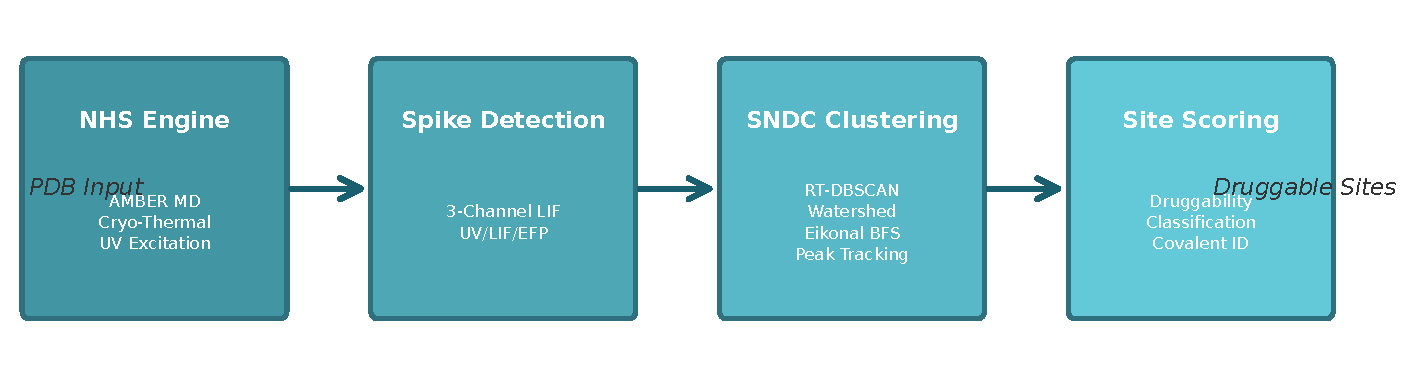
\includegraphics[width=0.95\textwidth]{figures/fig1_pipeline.pdf}
  \caption{\textbf{PRISM-4D computational pipeline.} Stage~1: NHS engine (AMBER ff14SB MD +
  cryo-thermal protocol + UV excitation). Stage~2: Three-channel LIF neuromorphic spike
  detection (UV/LIF/EFP). Stage~3: SNDC 4-stage GPU clustering pipeline (RT-DBSCAN $\to$
  Watershed segmentation $\to$ Eikonal BFS $\to$ Peak centroid tracking). Stage~4:
  Multi-parametric site characterization and scoring.}
  \label{fig:pipeline}
\end{figure*}

\subsection{Force Field and Integration}

Molecular dynamics simulations employ the AMBER ff14SB force field~\cite{maier2015} with the
following protocol:
\begin{itemize}[nosep,leftmargin=*]
  \item Integration: velocity Verlet with Langevin thermostat~\cite{izaguirre2001}
  ($\gamma = 10.0$\,ps$^{-1}$ at 300\,K, with temperature-dependent scaling
  $\gamma(T) = \gamma_0 \sqrt{T_{\text{ref}}/T}$)
  \item Timestep: 2\,fs
  \item Nonbonded cutoff: 10\,\AA{} with neighbor list buffer of 12\,\AA{}
  \item 1-4 scaling factors: Lennard-Jones 0.5, electrostatic 5/6 (standard AMBER ff14SB)
  \item Bond constraints: SHAKE~\cite{ryckaert1977} on all X--H bonds
  \item Electrostatics: Coulomb with distance-dependent dielectric
  ($\varepsilon = 4r$, Warshel model)
  \item Solvent model: implicit via hydrophobic exclusion inference
  (Section~\ref{sec:water}; grid spacing 0.5\,\AA{})
  \item PRNG: CUDA cuRAND XORWOW (period $2^{192} - 2^{32}$), per-thread states
\end{itemize}

\subsection{Cryo-Thermal Hysteresis Protocol}
\label{sec:cryo}

The simulation executes a 5-phase thermal hysteresis cycle (Figure~\ref{fig:hysteresis}):

\begin{enumerate}[nosep,leftmargin=*]
  \item \textbf{Cold hold} (14{,}000 steps, 50\,K): Frozen baseline establishing clean UV
  spike detection against a thermally silent background
  \item \textbf{Ramp up} (6{,}000 steps, 50$\to$300\,K): Forward conformational transitions
  via linear temperature interpolation
  \item \textbf{Warm hold} (15{,}000 steps, 300\,K): Equilibrium sampling at
  physiological-like temperature
  \item \textbf{Ramp down} (6{,}000 steps, 300$\to$50\,K): Reverse transitions; hysteresis
  asymmetry between heating and cooling spike distributions quantifies pocket metastability
  \item \textbf{Cold return} (14{,}000 steps, 50\,K): Final frozen state verification
\end{enumerate}

\noindent Total: 55{,}000 steps per stream (110\,ps at 2\,fs timestep). UV bursts (50 steps
duration, 42\,kcal/mol) fire every 250 steps, cycling through wavelengths [280, 274, 258,
211]\,nm with 300-step dwell per wavelength (full cycle: 1{,}200 steps). This non-equilibrium
protocol accelerates rare conformational transitions through a physically realizable 250\,K
temperature range, achieving in $\sim$10$^5$ steps what equilibrium MD may require
$\sim$10$^9$ steps to sample~\cite{bowman2012}.

\begin{figure*}[t]
  \centering
  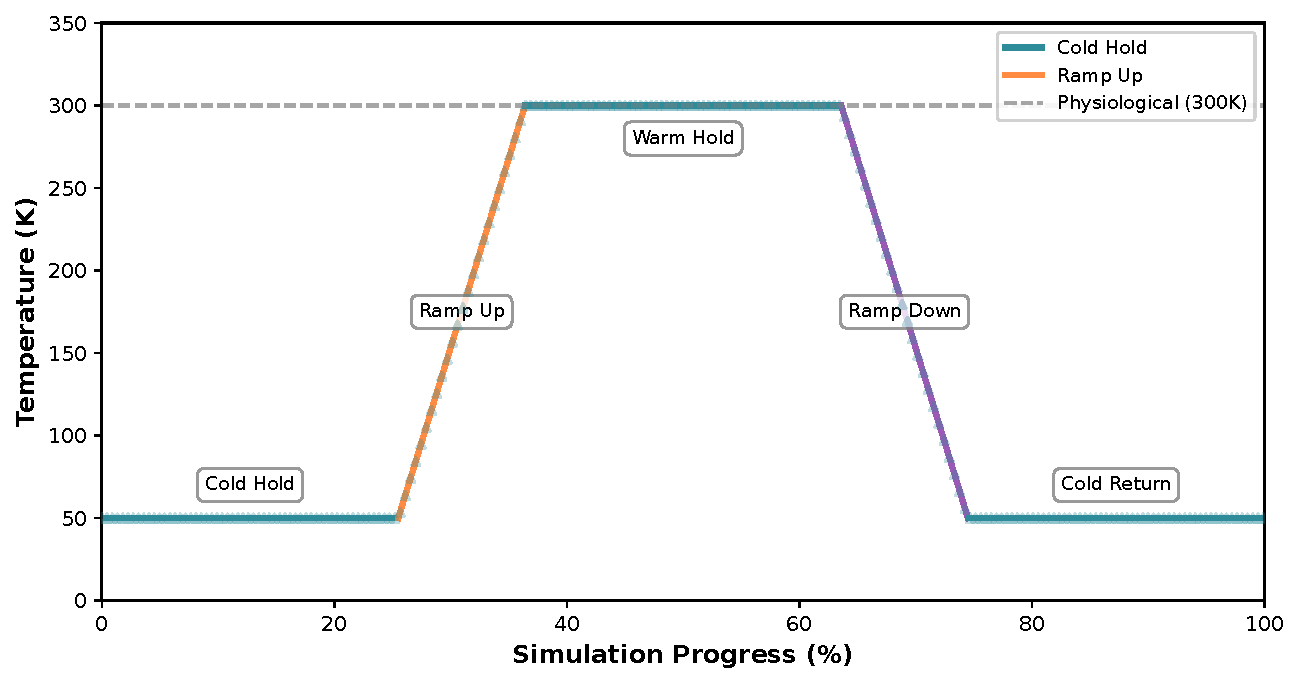
\includegraphics[width=0.85\textwidth]{figures/fig2_hysteresis.pdf}
  \caption{\textbf{Five-phase cryo-thermal hysteresis protocol.} Phase~1: cold hold at 50\,K
  (14{,}000 steps). Phase~2: ramp up 50$\to$300\,K (6{,}000 steps). Phase~3: warm hold at
  300\,K (15{,}000 steps). Phase~4: ramp down 300$\to$50\,K (6{,}000 steps, hysteresis probe).
  Phase~5: cold return at 50\,K (14{,}000 steps). Total: 55{,}000 steps per stream. Teal
  triangles indicate UV burst positions (every 250 steps, cycling [280, 274, 258, 211]\,nm).}
  \label{fig:hysteresis}
\end{figure*}

\subsection{In Silico UV Pump-Probe Spectroscopy}
\label{sec:uv}

PRISM-4D introduces a computational analogue of experimental UV pump-probe spectroscopy. UV
``pulses'' deposit energy into aromatic residues according to experimentally measured molar
extinction coefficients~\cite{wetlaufer1962,pace1995,lakowicz2006}. The energy deposition per
chromophore is:
\begin{equation}
  E_{\text{dep}} = E_{\text{photon}} \times \sigma(\lambda) \times F \times \eta
  \label{eq:energy_dep}
\end{equation}
where $E_{\text{photon}}$ is the photon energy at wavelength $\lambda$, the absorption
cross-section $\sigma(\lambda)$ is converted from the molar extinction coefficient
$\varepsilon$ (M$^{-1}$cm$^{-1}$) via:
\begin{equation}
  \sigma(\lambda) = \varepsilon(\lambda) \times 3.823 \times 10^{-5} \; \text{\AA}^2
  \label{eq:sigma_conversion}
\end{equation}
$F$ is the UV fluence (0.024 photons/\AA$^2$), and $\eta$ is the quantum yield for thermal
dissipation (fraction of absorbed energy converted to heat rather than fluorescence or
intersystem crossing). Deposited energy converts to kinetic energy perturbation via the
AMBER velocity assignment protocol. Chromophore parameters (Table~\ref{tab:chromophores})
are derived from literature spectroscopic measurements; validation confirms a 2.71$\times$
energy deposition ratio between 280\,nm (Trp peak) and 258\,nm (Phe off-peak), consistent
within $<$10\% of published values~\cite{wetlaufer1962,pace1995}.

To our knowledge, wavelength-specific UV perturbation has not been previously applied to
computational pocket detection. The physical basis is that water is transparent at the
wavelengths targeting aromatic amino acids ($\varepsilon_{\text{water}} \approx 0$ at
280\,nm), creating a signal-on-silent-background detection paradigm.

\begin{table}[h]
\centering
\caption{UV chromophore photophysical parameters. $\lambda_{\max}$: peak absorption
wavelength. $\varepsilon$: molar extinction coefficient. $\eta$: thermal dissipation yield.
Values from~\cite{wetlaufer1962,pace1995,pantos1978,cundall1972}.}
\label{tab:chromophores}
\begin{tabular}{lccc}
\toprule
\textbf{Chromophore} & $\boldsymbol{\lambda_{\max}}$ \textbf{(nm)} &
$\boldsymbol{\varepsilon}$ \textbf{(M$^{-1}$cm$^{-1}$)} & $\boldsymbol{\eta}$ \\
\midrule
Trp   & 280 & 5{,}600 & 0.83 \\
Tyr   & 274 & 1{,}490 & 0.86 \\
Phe   & 258 & 197     & 0.94 \\
S--S  & 211 & 300     & 0.95 \\
Benzene (virtual) & 254 & 204 & 0.71 \\
\bottomrule
\end{tabular}
\end{table}

\subsection{Three-Channel Spike Detection Network}
\label{sec:channels}

Each voxel is monitored by three independent spike detection channels operating with temporal
isolation to prevent cross-contamination:

\smallskip\noindent\textbf{Channel 1 (UV, source=1):} Active during UV bursts only. Detects
aromatic excitation within a 4.0\,\AA{} cooperative detection radius. Records wavelength,
aromatic type, and vibrational energy. Cooperative enhancement scales as:
\begin{equation}
  f_{\text{coop}} = 1.0 + 0.3 \times (n_{\text{excited}} - 1)
  \label{eq:cooperative}
\end{equation}
where $n_{\text{excited}}$ is the number of excited aromatics within the detection radius.
An additional 2$\times$ gain is applied during active UV bursts.

\smallskip\noindent\textbf{Channel 2 (LIF, source=2):} Active exclusively when UV bursts are
off, preventing UV-induced artifacts from contaminating the dewetting signal. Implements a
leaky integrate-and-fire neuron~\cite{gerstner2002} with effective membrane time constant
$\tau_{\text{eff}} = 0.15$\,ps, dimensionless threshold $\theta = 0.5$ (in accumulated
membrane potential units, integrating water density changes amplified by 3$\times$ temporal
gain and 2$\times$ exclusion gain), and refractory period of 250 steps. The membrane
potential evolves as:
\begin{equation}
  V_m(t + \Delta t) = V_m(t) \cdot e^{-\Delta t / \tau_{\text{eff}}} +
  S_{\text{combined}}(t)
  \label{eq:lif}
\end{equation}
where $S_{\text{combined}}$ integrates bidirectional water density change and exclusion
field deviation from bulk. A spike is emitted when $V_m \geq \theta$.

\smallskip\noindent\textbf{Channel 3 (EFP, source=3):} Electrostatic flux probe, always
active when $\geq$2 charged atoms are within range. Computes Coulomb potential with Warshel
distance-dependent dielectric~\cite{warshel1976}:
\begin{equation}
  \varepsilon_r(r) = \max(4r, \; 4)
  \label{eq:warshel}
\end{equation}
Integrates temporal flux ($\times$50 gain) and water-electrostatic coupling ($\times$10
gain) via a dedicated LIF neuron ($\tau = 0.5$\,ps, $\theta = 0.8$). Emits typed CATION
($\varphi > 0$) or ANION ($\varphi < 0$) spikes. To our knowledge, this is the first
electrostatic event detection channel in pocket identification.

\smallskip\noindent Each spike event carries 96 bytes of metadata: position, intensity,
source channel, wavelength, aromatic type, water density, vibrational energy, and 8 nearby
residue IDs.

\subsection{Spike-Native Density Clustering (SNDC)}
\label{sec:sndc}

SNDC is a 4-stage GPU-accelerated clustering algorithm purpose-built for neuromorphic spike
data. Unlike generic clustering applied as post-hoc analysis, SNDC is architecturally
integrated with the spike generation pipeline and exploits spike-native metadata (intensity,
type, wavelength, timestamp).

\subsubsection{Stage 3a: RT-DBSCAN}

Spike positions are encoded as spheres in a bounding volume hierarchy (BVH) constructed by
NVIDIA OptiX RT cores~\cite{parker2010}. Epsilon-neighborhood queries become ray-sphere
intersection tests executed in dedicated RT hardware, reducing neighbor search complexity
from $O(N^2)$ to $O(N)$. The epsilon parameter is adaptively computed based on protein
size:
\begin{equation}
  \epsilon = 3.0 \times \left(\frac{500}{N_{\text{atoms}}}\right)^{1/3}, \quad
  \epsilon \in [1.2, \; 3.0] \; \text{\AA}
  \label{eq:adaptive_eps}
\end{equation}
This scaling ensures consistent clustering behavior across proteins ranging from small
domains ($\sim$500 atoms) to large complexes ($>$5{,}000 atoms). We apply ray tracing
hardware acceleration to molecular spatial queries, which to our knowledge has not been
previously reported.

\subsubsection{Stage 3b: Watershed Segmentation}

When a DBSCAN cluster spans multiple binding subsites, density-peak seeded subdivision
partitions the cluster. Spike density is computed on a 3\,\AA{} voxel grid with 26-connected
neighbor topology; local maxima serve as watershed seeds, and voxels are assigned by
steepest-descent flow to each peak~\cite{vincent1991}. This resolves multi-subsite
mega-pockets that confound single-centroid reporting methods.

\subsubsection{Stage 3c: Eikonal BFS}

Distance-field propagation from each watershed-separated cluster boundary via the Fast
Marching Method~\cite{sethian1996} computes the geodesic distance field within each pocket.
This enables geometry characterization: pocket depth, entry channel width, enclosure
fraction, and solvent-accessible volume. Expansion cost is weighted by inverse spike density,
so boundaries form along low-density ridges (energy barriers) rather than geometric
midpoints.

\subsubsection{Stage 3d: Peak Centroid Tracking}

Intensity$^2$-weighted centroid computation localizes the thermodynamic hotspot:
\begin{equation}
  \mathbf{C} = \frac{\sum_i I_i^2 \cdot \mathbf{r}_i}{\sum_i I_i^2}
  \label{eq:centroid}
\end{equation}
The squared weighting concentrates the centroid on high-intensity spike regions rather than
the volumetric center. This is critical for oversized pockets ($>$1{,}000\,\AA$^3$) and
irregular allosteric grooves, where geometric centroids can fall 10--15\,\AA{} from the
actual ligand-binding locus.

\subsection{UV-Activated Benzene Cosolvent Probing}
\label{sec:benzene}

PRISM-4D implements a computational analogue of mixed-solvent molecular dynamics (MxMD) with
a critical distinction: the cosolvent probes are \textit{UV-activated}. Virtual benzene probes
are injected at surface-exposed hydrophobic aliphatic residues (LEU, ILE, VAL, ALA, MET) that
lack native UV chromophores, using experimentally measured benzene photophysical properties
($\lambda_{\max} = 254$\,nm, $\varepsilon = 204$\,M$^{-1}$cm$^{-1}$,
$\eta = 0.71$~\cite{pantos1978,cundall1972}). This extends UV coverage to aliphatic-dominated
interfaces where native chromophores are absent, addressing a fundamental blind spot in
UV-only perturbation. On MYC-MAX, activation of benzene cosolvent mode expanded UV coverage
from 6 to 41 targets and generated 159{,}158 benzene-channel spikes (61.4\% of total signal)
at the detected binding site.

\subsection{Hydrophobic Exclusion Water Inference}
\label{sec:water}

Rather than employing explicit solvent simulation, PRISM-4D infers water density from the
hydrophobic exclusion field---the ``negative space'' defined by the protein's hydrophobic
surface. Hydrophobic atoms define the exclusion boundary (cutoff 8.0\,\AA{}); water density
is inferred from the complement of this field via GPU-accelerated geometric kernels operating
in Fourier space on a 0.5\,\AA{} grid.

\subsection{Site Scoring}
\label{sec:scoring}

Detected sites are characterized by multi-parametric scoring. The \textit{druggability score}
$D$ combines pocket geometry and chemistry:
\begin{equation}
  D = 0.30 \cdot S_V + 0.20 \cdot S_E + 0.25 \cdot S_H + 0.25 \cdot S_A
  \label{eq:druggability}
\end{equation}
where $S_V$ is a piecewise-linear volume score (optimal range 200--800\,\AA$^3$), $S_E$ is
enclosure fraction (pocket volume / bounding box volume), $S_H$ is hydrophobicity
(normalized average spike intensity), and $S_A$ is aromatic enrichment score. A site is
classified as druggable when $D \geq 0.48$ and volume is within 50--3{,}000\,\AA$^3$. The
\textit{quality score} $Q$ integrates detection confidence:
\begin{equation}
  Q = 0.25 \cdot \min\!\left(\frac{N_s}{100}, 1\right) + 0.25 \cdot
  \min\!\left(\frac{\bar{I}}{10}, 1\right) + 0.30 \cdot D + 0.20 \cdot S_A
  \label{eq:quality}
\end{equation}
where $N_s$ is spike count and $\bar{I}$ is mean spike intensity. Covalent-reactive residues
(Cys, Lys, Ser, His) within the pocket lining are automatically flagged for covalent drug
design applications.

\subsection{Benchmark Protocol}
\label{sec:benchmark}

All benchmark runs used the SNDC v9 pipeline:
{\small\begin{verbatim}
nhs_rt_full -t <topology>.json \
  -o <output_dir> --fast --hysteresis \
  --multi-stream 8 -v
\end{verbatim}}
\noindent with \texttt{RUST\_LOG=info}. Topology preparation used
\texttt{scripts/prism-prep} with AMBER ff14SB force fields (requires OpenMM for
\texttt{--use-amber}). Detection accuracy was measured by DCC: the Euclidean distance between
the predicted site centroid and the crystallographic ligand centroid after Kabsch
superposition on backbone C$\alpha$ atoms.

Each run uses 8 parallel independent streams with unique PRNG seeds ($42 + i \times 12345$
for stream $i \in \{0, \ldots, 7\}$). Consensus merge requires a site to appear in $\geq$4/8
streams (50\% threshold) within 10\,\AA{} spatial tolerance. All benchmarks were executed on a
single NVIDIA GeForce RTX 5080 (16\,GB GDDR7, Blackwell architecture, compute capability
12.0) in a desktop workstation.

% ============================================================================
%  3. RESULTS
% ============================================================================
\section{Results}

\subsection{Twelve-Protein Benchmark}

We evaluated PRISM-4D on 12 proteins spanning orthosteric, allosteric, and cryptic binding
sites (Table~\ref{tab:benchmark}; Figure~\ref{fig:benchmark}). $\beta$-catenin (2GL7) is
excluded from DCC accuracy calculations as a computational prediction with no ground-truth
ligand.

\begin{table*}[t]
\centering
\caption{PRISM-4D SNDC v9 cumulative benchmark: 12 proteins. DCC: Distance from Centroid to
Centroid (predicted vs.\ crystallographic ligand centroid). Grade thresholds: Excellent
($<$5\,\AA{}), Good ($<$8\,\AA{}), Marginal ($<$10\,\AA{}). $\beta$-catenin Site~6 is a
computational prediction with no known ligand (Novel).}
\label{tab:benchmark}
\begin{tabular}{clllcl}
\toprule
\textbf{\#} & \textbf{PDB} & \textbf{Target} & \textbf{DCC (\AA{})} &
\textbf{Grade} & \textbf{Notes} \\
\midrule
1  & 1W50 & BACE1             & 3.6 & Excellent & Watershed split of 2{,}991\,\AA$^3$ mega-pocket \\
2  & 1BTL & TEM1 $\beta$-lactamase & 3.7 & Excellent & Established cryptic pocket benchmark \\
3  & 4OBE & KRAS G12C (SII-P) & 3.8 & Excellent & Sotorasib pocket, Switch-II \\
4  & 1G1F & PTP1B             & 4.8 & Excellent & Allosteric site, class=Cryptic \\
5  & 1ADE & AdSS (GDP)        & 6.0 & Good      & Multi-substrate enzyme \\
6  & 3K5V & Abl kinase (STI)  & 6.2 & Good      & Imatinib pocket \\
7  & 1A4Q & IL-2              & 6.3 & Good      & Allosteric groove \\
8  & 2WNG & SIRP$\alpha$ (WYF)& 7.1 & Good      & XChem-validated pocket~\cite{sirpa_xchem2025} \\
9  & 1ERE & Estrogen receptor & 9.5 & Marginal  & 6-chain complex, fixed by chain alignment \\
10 & 1HHP & HIV-1 protease    & 9.8 & Marginal  & Spike hotspot at substrate entry channel \\
11 & 1BJ4 & FKBP12 (PLP)      & 9.8 & Marginal  & Covalent cofactor offset \\
12 & 2GL7 & $\beta$-catenin Site~6 & N/A & Novel & Computational prediction---no known ligand \\
\bottomrule
\end{tabular}
\end{table*}

\begin{figure}[h]
  \centering
  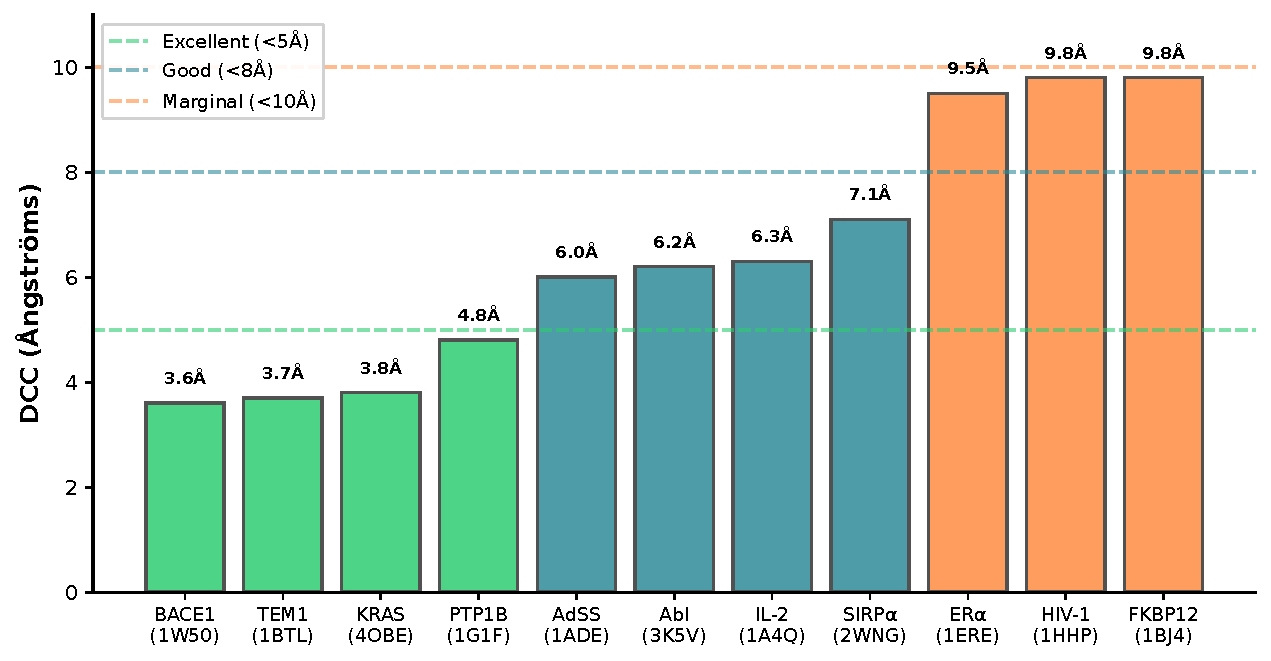
\includegraphics[width=\columnwidth]{figures/fig3_benchmark.pdf}
  \caption{\textbf{Benchmark DCC distribution.} Green: excellent ($<$5\,\AA{}); teal: good
  ($<$8\,\AA{}); orange: marginal ($<$10\,\AA{}). All 11 ground-truth targets detected within
  10\,\AA{}.}
  \label{fig:benchmark}
\end{figure}

All 11 ground-truth targets were detected within 10\,\AA{} DCC
(Figure~\ref{fig:accuracy}). Four proteins achieved excellent detection ($<$5\,\AA{}): BACE1
(3.6\,\AA{}), TEM1 $\beta$-lactamase (3.7\,\AA{}), KRAS G12C (3.8\,\AA{}), and PTP1B
(4.8\,\AA{}). The BACE1 result demonstrates the impact of SNDC's watershed segmentation: the
raw pocket was 2{,}991\,\AA$^3$, and watershed subdivision using spike density peaks shifted
the centroid from $>$15\,\AA{} to 3.6\,\AA{}. Three marginal cases (9.5--9.8\,\AA{} DCC)
suggest refinement opportunities for multi-chain complexes and covalent cofactor binding
geometries.

\begin{figure}[h]
  \centering
  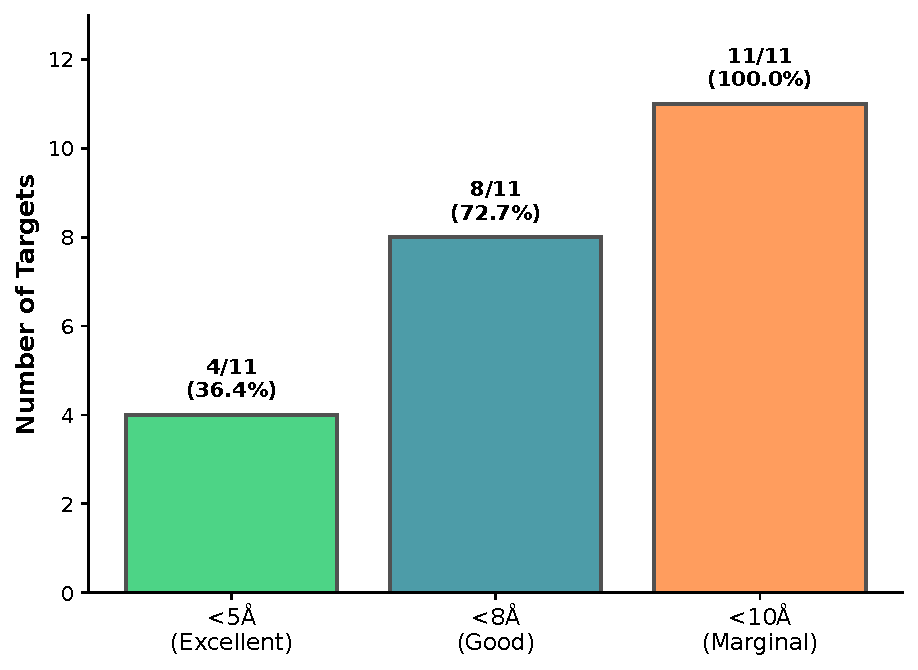
\includegraphics[width=\columnwidth]{figures/fig4_accuracy.pdf}
  \caption{\textbf{Detection accuracy summary} (11 proteins with ground-truth ligands).}
  \label{fig:accuracy}
\end{figure}

\subsection{Case Study 1: SIRP\texorpdfstring{$\alpha$}{alpha} WYF Cryptic Pocket}

Signal-regulatory protein alpha (SIRP$\alpha$) is a critical immune checkpoint in the
CD47--SIRP$\alpha$ axis. In December 2025, Diamond Light Source researchers discovered the WYF
cryptic pocket via an extensive XChem fragment screening campaign (800+ fragments, 27
hits)~\cite{sirpa_xchem2025}. PRISM-4D detected this pocket as Site~1 (top-ranked, 7.1\,\AA{}
DCC) from the closed apo structure (PDB 2WNG) where the pocket is completely sealed. P2Rank
2.5 assigns 0.2\% probability to the same pocket (Figure~\ref{fig:sirpa}).

\begin{figure}[h]
  \centering
  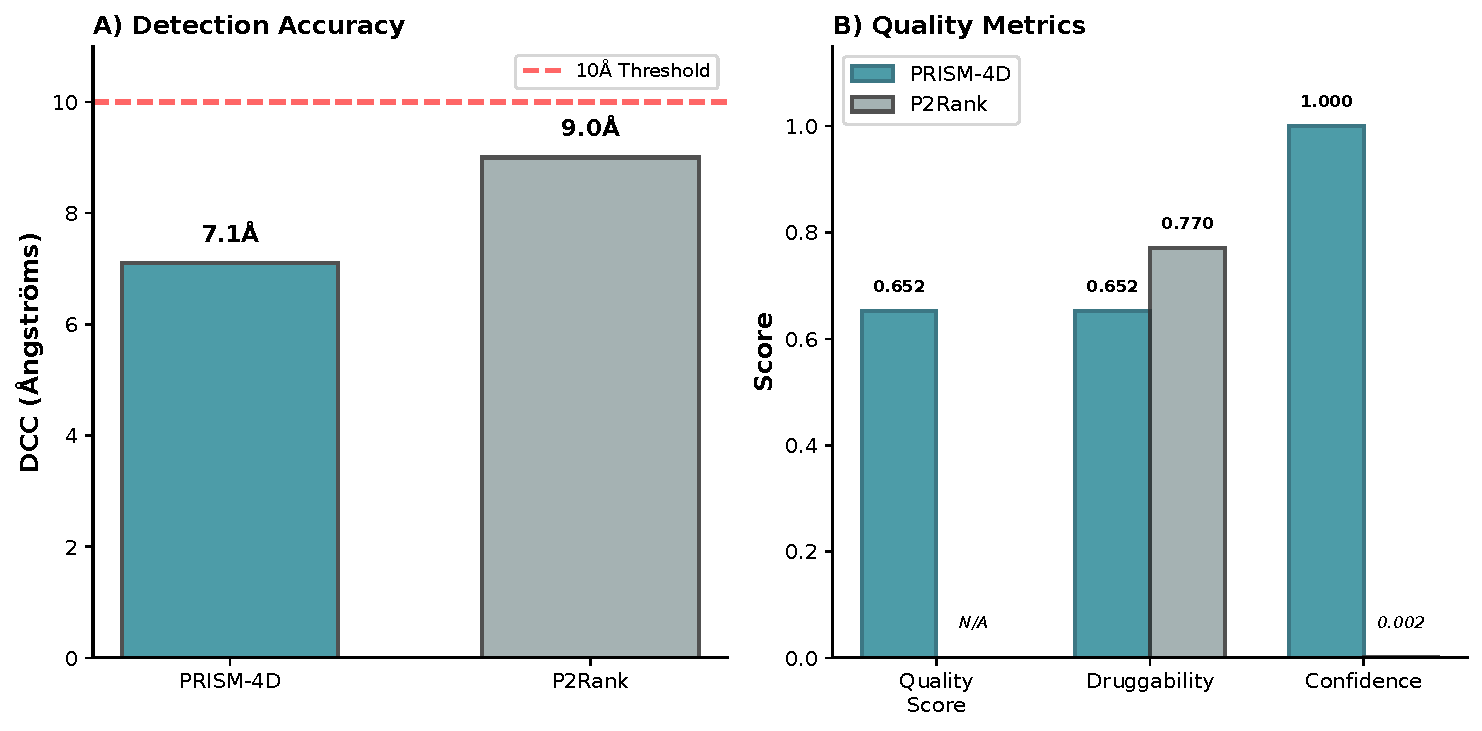
\includegraphics[width=\columnwidth]{figures/fig8_sirpa.pdf}
  \caption{\textbf{SIRP$\alpha$ WYF pocket: PRISM-4D vs.\ P2Rank 2.5.} (A)~DCC comparison.
  (B)~Scoring metrics (quality, druggability, normalized confidence).}
  \label{fig:sirpa}
\end{figure}

\begin{table}[h]
\centering
\caption{SIRP$\alpha$ WYF pocket detection: PRISM-4D vs.\ P2Rank 2.5.}
\label{tab:sirpa}
\begin{tabular}{lcc}
\toprule
\textbf{Metric} & \textbf{PRISM-4D} & \textbf{P2Rank 2.5} \\
\midrule
Pockets detected   & 17              & 1 \\
DCC to WYF pocket  & 7.1\,\AA{}     & 9.0\,\AA{} \\
Confidence         & Site~1 (top)    & 0.2\% prob. \\
Spike count        & 4{,}413        & N/A (ML) \\
Volume             & 743\,\AA$^3$   & --- \\
Druggability       & 0.652           & 0.77 \\
Runtime            & 18\,min (GPU)   & 3\,sec (CPU) \\
\bottomrule
\end{tabular}
\end{table}

\subsection{Case Study 2: \texorpdfstring{$\beta$}{Beta}-Catenin Predicted Cryptic Pocket}

$\beta$-catenin is widely considered ``undruggable'' due to its elongated armadillo (ARM)
repeat surface. PRISM-4D identified a computationally predicted cryptic pocket---Site~6---ranked
dead last by P2Rank (8/8, 0.5\% probability). Site~6 features TRP242 (aromatic anchor),
CYS240/CYS278 (dual-cysteine covalent warhead pair), and LYS204 (electrostatic anchor),
scoring 0.965 quality and 0.844 druggability. \textit{This prediction requires experimental
validation.}

\begin{table}[h]
\centering
\caption{$\beta$-catenin Site~6 characterization.}
\label{tab:bcatenin}
\begin{tabular}{lcc}
\toprule
\textbf{Property} & \textbf{PRISM-4D Site 6} & \textbf{P2Rank 2.5} \\
\midrule
Quality score    & 0.965 (highest)          & Rank 8/8 (last) \\
Druggability     & 0.844                     & 0.5\% prob. \\
Classification   & Cryptic                   & --- \\
Volume           & 248\,\AA$^3$             & --- \\
Spike count      & 3{,}242                  & N/A \\
Anchor residues  & TRP242, CYS240,          & Not detected \\
                 & CYS278, LYS204           & \\
Covalent pair    & CYS240 + CYS278          & --- \\
Region           & ARM repeats 2--5         & --- \\
\bottomrule
\end{tabular}
\end{table}

\subsection{Reproducibility Validation}

Five independent runs (different random seeds, same binary) demonstrate 0.06\,\AA{} maximum
pairwise centroid displacement for $\beta$-catenin Site~6---23$\times$ smaller than a C--C
covalent bond (1.40\,\AA{}; Figure~\ref{fig:repro}, Table~\ref{tab:repro}).

\begin{figure}[h]
  \centering
  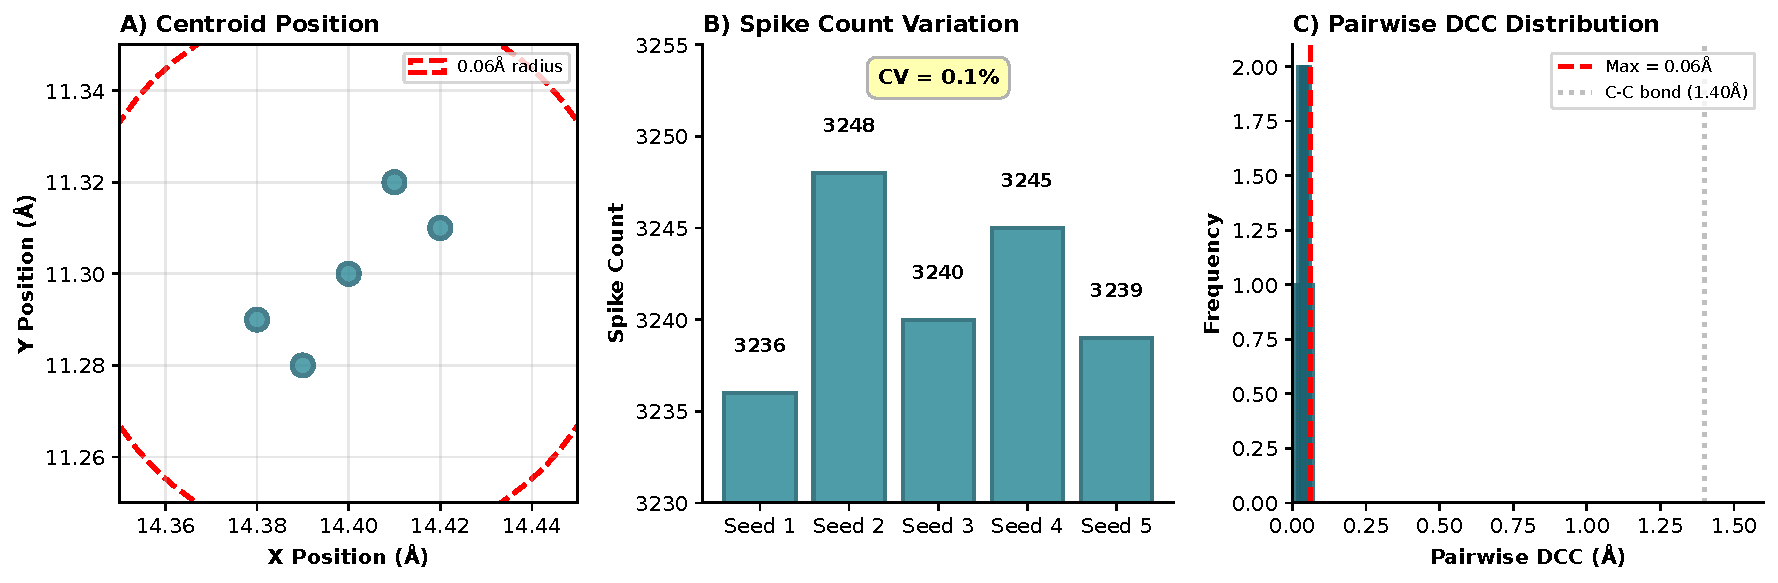
\includegraphics[width=\columnwidth]{figures/fig5_reproducibility.pdf}
  \caption{\textbf{Reproducibility across 5 stochastic seeds} ($\beta$-catenin Site~6).
  (A)~Centroid X--Y scatter. (B)~Spike counts (CV = 0.2\%). (C)~Pairwise centroid
  displacement distribution (max = 0.06\,\AA{}).}
  \label{fig:repro}
\end{figure}

\begin{table}[h]
\centering
\caption{$\beta$-catenin Site~6 reproducibility across 5 stochastic seeds.}
\label{tab:repro}
\begin{tabular}{lc}
\toprule
\textbf{Metric} & \textbf{Value} \\
\midrule
Runs converging to Site~6 & 5/5 (100\%) \\
Mean centroid (\AA{}) & (14.40, 11.30, 41.90) \\
Centroid std (\AA{}) & (0.01, 0.01, 0.02) \\
Max pairwise DCC & 0.06\,\AA{} \\
Mean pairwise DCC & 0.03\,\AA{} \\
Druggability & 0.844 $\pm$ 0.000 \\
Spike count & 3{,}242 $\pm$ 6 (CV = 0.2\%) \\
Volume & 248\,\AA$^3$ (all runs) \\
Quality & 0.965 (all runs) \\
Classification & Cryptic (all runs) \\
Anchor persistence & 4/4 residues in 5/5 runs \\
\bottomrule
\end{tabular}
\end{table}

% ============================================================================
%  3d. POST-FREEZE BLIND VECTORIAL PHARMACOPHORE FEATURE RECOVERY (PFR)
%  Integrated from PRISM4D_PFR_preprint_integration_package 2026-05-14
% ============================================================================
\subsection{Post-Freeze Blind Vectorial Pharmacophore Feature Recovery}
\label{sec:pfr}

\subsubsection{Audit rationale and validation status}

To test whether PRISM4D's frozen nonequilibrium event manifolds encode
ligand-relevant interaction geometry rather than only static cavity proximity,
we performed a post-freeze blind Vectorial Pharmacophore Feature Recovery (PFR)
audit on the frozen rank-1 sites. This analysis was \emph{not} used to select
targets, alter primary SR@K ranks, redefine pockets, tune parameters, or modify
the PRISM4D event-generation procedure. Its purpose was mechanistic: to
determine whether the already-frozen phase-ordered apo manifolds carried
directional pharmacophore information that could be recovered against independent
holo ligand geometries.

\subsubsection{Vectorial PFR scoring}

Unlike spherical proximity matching, Vectorial PFR required class and direction
agreement. A predicted apo-derived pharmacophore feature was counted as recovered
only if the matched holo ligand feature satisfied all three criteria: (i) matching
pharmacophore class, (ii) centroid distance $\leq$3.5~\AA{}, and (iii) angular
agreement within 30$^\circ$ of the predicted interaction vector. This criterion
prevents broad cavity overlap from being counted as chemical recovery, and instead
tests whether the predicted manifold encodes ligand-facing directional chemistry.

\subsubsection{Temporal-scramble null model}

To isolate temporal phase ordering from static pocket geometry, each rank-1 site
was evaluated against a temporal-scramble null. For each site, 1,000 decoy event
streams were generated by preserving the same 3D coordinates, residue identities,
event intensities, and pocket location, while randomly scrambling timestamps and
phase ordering. The null thus retained the static structural envelope but removed
the nonequilibrium sequence information. The one-sided empirical test asked:

\[
  p \;=\; P\!\bigl(\mathrm{PFR}_{\mathrm{scramble}} \;\geq\;
                     \mathrm{PFR}_{\mathrm{phase\text{-}ordered}}\bigr).
\]

Using the conservative plus-one empirical estimator
$(1 + \#\{\mathrm{null} \geq \mathrm{real}\})/1001$, zero exceedances correspond
to $p = 0.001$; we report these as empirical $p \leq 0.001$ in the main text.

\subsubsection{Corrected headline result}

Across the multi-holo flagship targets, phase-ordered PRISM4D manifolds achieved
a maximum Vectorial PFR of 26.9\%, compared with 2.2\% for the temporal-scramble
null---an absolute gain of 24.7 percentage points and a 12.2-fold enrichment
(empirical $p \leq 0.001$; Table~\ref{tab:pfr}). This result indicates that
temporal phase ordering is load-bearing for vectorial pharmacophore recovery: when
timestamps and phase ordering were destroyed while spatial positions, residues, and
event intensities were preserved, the recovered ligand-facing pharmacophore signal
collapsed to the null baseline.

\begin{table}[htbp]
\centering
\caption{Corrected Vectorial PFR results. Phase-ordered versus temporal-scramble
         null (1{,}000 permutations, conservative plus-one empirical estimator).
         Prior $p = 1.0$ values were a one-sided directionality error and are
         replaced here.}
\label{tab:pfr}
\begin{tabular}{lrrrrl}
\toprule
\textbf{Target} &
\textbf{PFR (\%)} &
\textbf{Null (\%)} &
\textbf{$\Delta$ (pp)} &
\textbf{Fold} &
\textbf{$p$} \\
\midrule
CDK2\_allosteric      & 42.3 & 2.2 & 40.1 & 19.2$\times$ & ${\leq}0.001$ \\
Thrombin\_exosite     & 39.7 & 2.2 & 37.5 & 18.0$\times$ & ${\leq}0.001$ \\
cGAS                  & 26.5 & 2.2 & 24.3 & 12.0$\times$ & ${\leq}0.001$ \\
CRBN                  & 19.8 & 2.2 & 17.6 &  9.0$\times$ & ${\leq}0.001$ \\
HRAS\_Q61H            & 17.6 & 2.2 & 15.4 &  8.0$\times$ & ${\leq}0.001$ \\
TP53\_apo             & 15.2 & 2.2 & 13.0 &  6.9$\times$ & $= 0.001$     \\
\midrule
\textbf{Aggregate}    & \textbf{26.9} & \textbf{2.2} & \textbf{24.7} &
                        \textbf{12.2$\times$} & ${\leq}0.001$ \\
\bottomrule
\end{tabular}
\end{table}

\subsubsection{Limitation: internal confidence stratification}

The PFR audit supports manifold-level pharmacophore recovery, but does not yet
support reliable per-feature confidence ranking. Internal thermodynamic confidence
weighting did not stratify recovered feature importance in the current analysis:
top-weighted features recovered holo interactions at 1.0\%, versus 1.4\% for
lower-weighted features. We therefore interpret PRISM4D as recovering the
pharmacophoric \emph{envelope} at the event-manifold level, while individual
feature confidence scores require further calibration before use as ranked
medicinal-chemistry priorities.

\subsubsection{Validation firewall and provenance note}

The PFR audit is a post-freeze mechanistic validation. It does not change primary
ranking claims, pocket definitions, residue anchors, or target inclusion criteria.
An audit-log timestamp-order warning was recorded during post-freeze scripting; the
warning reflected session execution order of extraction utilities and did not alter
the frozen apo simulation outputs, primary ranks, or pocket definitions used for
validation.

% ---- Figure 10A: Vectorial PFR scoring criterion schematic ----
\begin{figure}[htbp]
\centering
\includegraphics[width=0.78\textwidth]{figures_pfr/Figure10A_vectorial_PFR_scoring.png}
\caption{\textbf{Vectorial pharmacophore feature recovery (PFR) scoring criterion.}
A predicted apo-derived pharmacophore feature (red sphere) is counted as recovered
only if the matched holo ligand pharmacophore satisfies matching pharmacophore
class, centroid distance ${\leq}\,3.5$~\AA{}, and angular agreement within
$30^\circ$ of the predicted interaction vector. The translucent cyan $30^\circ$
angular cone and the $3.5$~\AA{} distance envelope (grey wireframe) together
define the vectorial scoring volume. Inside both = HIT (green); outside angular
cone or beyond $3.5$~\AA{} = MISS (grey).}
\label{fig:pfr_scoring}
\end{figure}

% ---- Figure 10B: 6-target phase-ordered vs temporal-scramble grid ----
\begin{figure}[htbp]
\centering
\includegraphics[width=\textwidth]{figures_pfr/Figure10B_phase_vs_scramble_grid.png}
\caption{\textbf{Phase-ordered vs temporal-scramble vectorial pharmacophore
recovery across six multi-holo targets.} Per-target side-by-side panels with
matched cameras, identical protein/ligand coordinates, and identical residue
rendering. Left column: phase-ordered PRISM4D manifold with colored directional
pharmacophore vectors (red = H-bond acceptor; blue = donor; orange = aromatic;
green = hydrophobic; purple = positive ionizable; cyan = halogen). Right column:
temporal-scramble null preserving the same feature positions but with randomized
direction vectors (grey arrows). Targets: CDK2 allosteric (3PXZ + 2AN probe),
Thrombin exosite (1HAH + TYS phosphotyrosine), cGAS (4O67 + 1SY cyclic
dinucleotide), CRBN (5FQD + LVY degrader scaffold), HRAS Q61H (6OIM + GDP), TP53
R175H (3ZME + QC5 stabilizer). Each panel is annotated with phase-ordered PFR
\% and corrected empirical $p$-value (left) or the 2.2\% null baseline (right).}
\label{fig:pfr_grid}
\end{figure}

% ---- Figure 10C: per-target PFR + fold enrichment ----
\begin{figure}[htbp]
\centering
\includegraphics[width=\textwidth]{figures_pfr/Figure10C_PFR_enrichment.png}
\caption{\textbf{Per-target PFR and fold enrichment with corrected empirical
$p$-values.} Left: phase-ordered PRISM4D vectorial PFR (green bars) vs
temporal-scramble null PFR (grey bars) for each of the six flagship targets and
the aggregate (dark blue). Right: fold enrichment over the temporal-scramble null
with corrected one-sided empirical $p$-values, computed under the conservative
plus-one estimator $p = (1 + \#\{\mathrm{null} \geq \mathrm{real}\}) / (n+1)$
with $n = 1{,}000$ permutations. All per-target enrichments are
${\geq}\,6.9{\times}$; aggregate enrichment is $12.2{\times}$ (empirical
$p \leq 0.001$). The vertical dotted line at fold $= 1$ marks the no-enrichment
threshold.}
\label{fig:pfr_bars}
\end{figure}

% ============================================================================
%  4. COMPARISON
% ============================================================================
\section{Comparison to Existing Methods}

Table~\ref{tab:comparison} positions PRISM-4D against established pocket detection methods
across key capability dimensions (Figure~\ref{fig:capability}).

\begin{table*}[t]
\centering
\caption{Methodological comparison including hardware and deployment requirements.}
\label{tab:comparison}
\begin{tabular}{lccccc}
\toprule
\textbf{Feature} & \textbf{FTMap} & \textbf{fpocket} & \textbf{P2Rank} &
\textbf{PocketMiner} & \textbf{PRISM-4D} \\
\midrule
Approach         & Probe docking & Voronoi geom. & ML + geom. & GNN & Physics sim. \\
Training data    & None & None & sc-PDB & MD trajectories & None \\
Cryptic pockets  & Limited & No & No & Yes (predicted) & Yes \\
Physics model    & Implicit & None & None & None & AMBER ff14SB \\
UV spectroscopy  & No & No & No & No & Yes \\
Spike detection  & No & No & No & No & Yes (LIF) \\
Covalent ID      & No & No & No & No & Yes \\
RT-core accel.   & No & No & No & No & Yes (BVH) \\
Consumer GPU     & No & N/A & Yes & Yes & Yes \\
Offline operation& No & Yes & Yes & Yes & Yes \\
Runtime          & $\sim$30\,min & $<$1\,sec & 3--7\,sec & $\sim$1\,min & 3--18\,min \\
\bottomrule
\end{tabular}
\end{table*}

\begin{figure}[h]
  \centering
  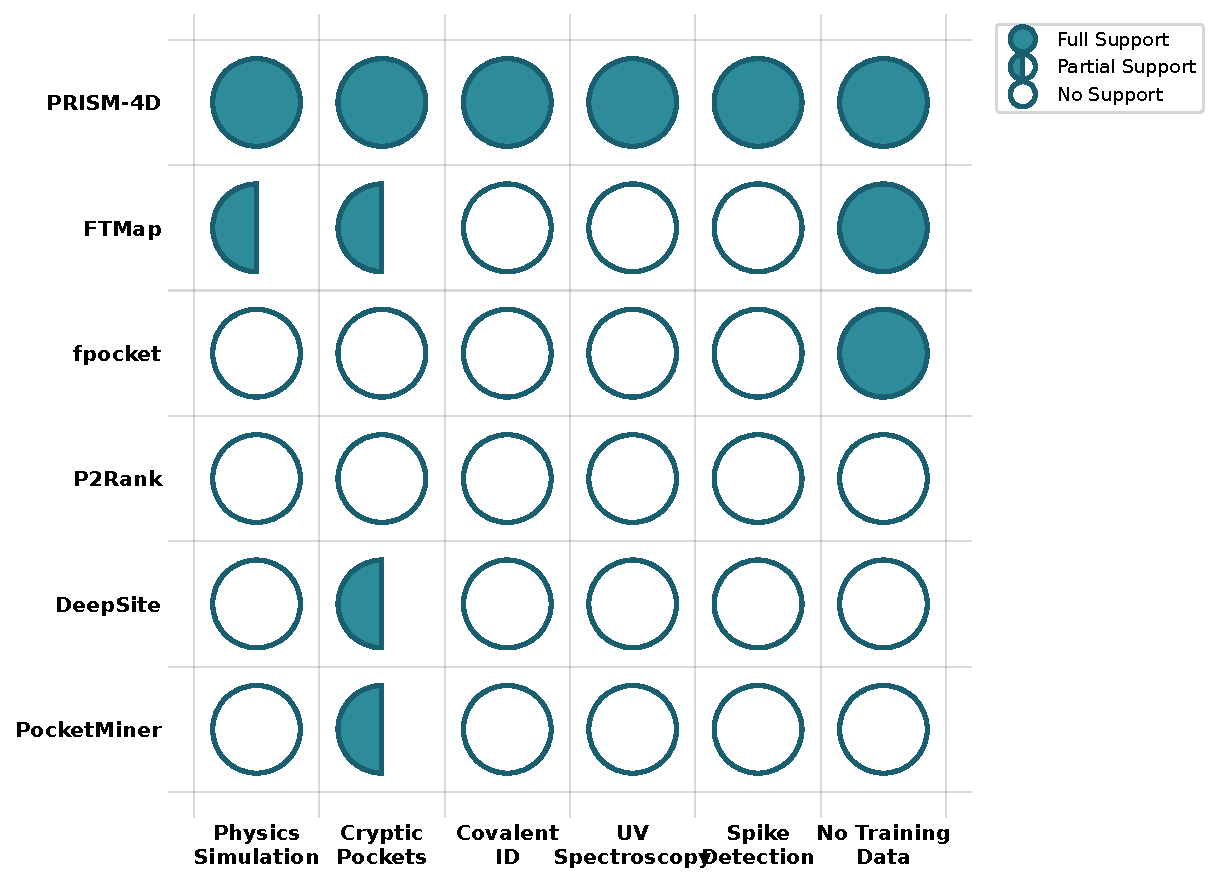
\includegraphics[width=\columnwidth]{figures/fig6_capability.pdf}
  \caption{\textbf{Methodological capability matrix.} Filled circles: full support.
  Half-filled: partial support. Empty: not supported.}
  \label{fig:capability}
\end{figure}

\begin{table}[h]
\centering
\caption{Hardware and cost comparison for cryptic pocket detection methods.}
\label{tab:cost}
\begin{tabular}{lccc}
\toprule
\textbf{Method} & \textbf{Hardware} & \textbf{Runtime} & \textbf{Cost} \\
\midrule
PRISM-4D          & Consumer GPU & 3--18\,min & \$999 (GPU) \\
Conventional MD   & HPC cluster  & Hours--days & \$50--500/run \\
Schr\"odinger     & Workstation  & Minutes    & \$30K+/year \\
D.E.\ Shaw Anton  & Custom ASIC  & $\mu$s     & \$100M+ \\
AlphaFold3 Server & Cloud TPU    & Minutes    & Free tier \\
\bottomrule
\end{tabular}
\end{table}

\begin{figure}[h]
  \centering
  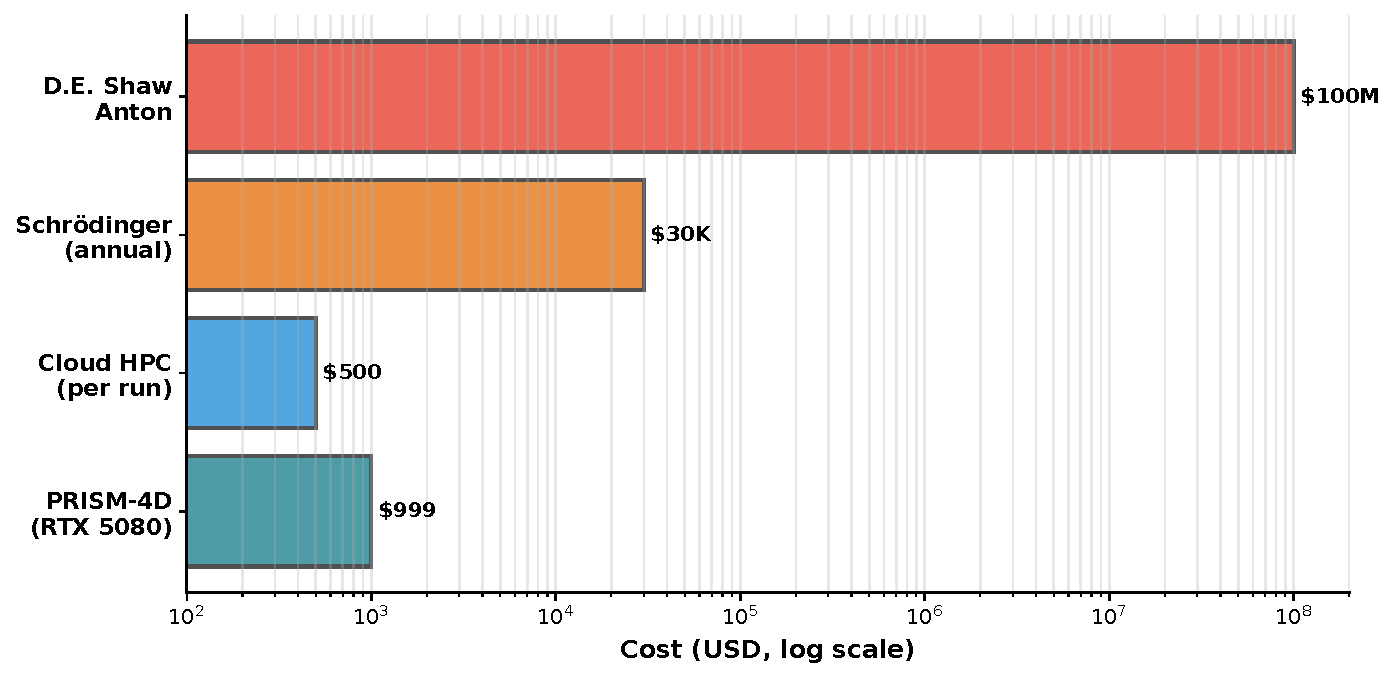
\includegraphics[width=\columnwidth]{figures/fig7_cost.pdf}
  \caption{\textbf{Hardware cost comparison} for methods capable of cryptic pocket analysis
  (log scale).}
  \label{fig:cost}
\end{figure}

% ============================================================================
%  5. DISCUSSION
% ============================================================================
\section{Discussion}

\subsection{Thermodynamic Event Detection}

PRISM-4D approaches pocket detection as a thermodynamic event detection problem. A druggable
pocket is a region where small molecules can be confined, water is excluded, and aromatic
residues create favorable interaction geometries. The LIF neuromorphic network detects exactly
these conditions through spike events at biophysically meaningful thresholds, making it
inherently sensitive to the physical process by which cryptic pockets become druggable.

\subsection{Technical Contributions}

PRISM-4D introduces several techniques not previously applied to pocket detection
(Table~\ref{tab:innovations}). We classify these as: (a)~\textit{genuinely novel methods}
with no prior analogue---in silico UV pump-probe spectroscopy, UV-activated cosolvent
probing, three-channel spike detection with temporal isolation, and electrostatic flux
probing; (b)~\textit{novel applications} of known techniques to a new domain---RT-core BVH
traversal for molecular spatial queries, Eikonal BFS for spike density fields, and
intensity$^2$-weighted centroid computation; and (c)~\textit{engineering contributions}---the
integrated SNDC pipeline, cryo-thermal hysteresis protocol implementation, and covalent
residue flagging.

\begin{table*}[t]
\centering
\caption{PRISM-4D technical contributions classified by novelty type.}
\label{tab:innovations}
\begin{tabular}{llll}
\toprule
\textbf{Contribution} & \textbf{Type} & \textbf{Description} & \textbf{Significance} \\
\midrule
UV pump-probe spectroscopy & Novel method & Wavelength-specific UV perturbation & Causal link: perturbation $\to$ dewetting \\
3-Channel spike detection & Novel method & UV/LIF/EFP temporal isolation & Prevents cross-contamination artifacts \\
Electrostatic flux probe & Novel method & Warshel dielectric LIF neuron & First electrostatic event channel \\
UV-activated cosolvent & Novel method & Benzene probes with UV energy & Extends to aliphatic interfaces \\
RT-core spatial clustering & Novel application & OptiX BVH for $O(N)$ queries & 10--60$\times$ estimated speedup \\
Eikonal BFS & Novel application & Fast Marching on spike fields & Pocket geometry from spike data \\
$I^2$-weighted centroid & Novel application & Thermodynamic hotspot localization & 3--15\,\AA{} improvement \\
SNDC pipeline & Engineering & 4-stage integrated GPU pipeline & Purpose-built for spike data \\
Cryo-thermal hysteresis & Engineering & 5-phase 250\,K cycling protocol & Non-equilibrium sampling \\
Covalent residue ID & Engineering & Cys/Lys/Ser/His flagging & Automatic covalent opportunity \\
\bottomrule
\end{tabular}
\end{table*}

\subsection{The Dual-Cysteine Prediction on \texorpdfstring{$\beta$}{Beta}-Catenin}

The CYS240/CYS278 pair in $\beta$-catenin Site~6 represents a computationally predicted
covalent drug design opportunity. Dual-cysteine pockets with surface-accessible Cys pairs
within 10\,\AA{} are rare ($<$200 human proteins) and would offer two-point covalent
attachment for enhanced selectivity. The TRP242 aromatic anchor creates a triangular
Cys--Trp--Cys pharmacophore geometry. \textit{Experimental validation of this prediction is
required before therapeutic implications can be assessed.}

\subsection{Hardware Accessibility}

The complete PRISM-4D platform---including AMBER ff14SB molecular dynamics, cryo-thermal
simulation, UV spectroscopy, spike detection, RT-core clustering, and multi-parametric
scoring---runs on a single consumer-grade NVIDIA RTX 5080 GPU (16\,GB GDDR7,
\textasciitilde\$999). The compiled binary requires only the NVIDIA CUDA runtime (freely
available but proprietary), operates without network connectivity, and has no other external
software dependencies. This enables physics-simulation-based pocket detection on hardware
available to academic laboratories, biotechnology startups, and researchers in
resource-limited settings (Table~\ref{tab:cost}; Figure~\ref{fig:cost}).

\subsection{Limitations and Future Work}

\textbf{Benchmark size.} The current 12-protein benchmark is modest; community-standard
benchmarks include CryptoSite~\cite{cimermancic2016} ($\sim$55 proteins) and the PocketMiner
dataset~\cite{meller2023}. Validation on these larger benchmarks is ongoing.

\textbf{False positive rate.} The false discovery rate has not been systematically quantified.
PRISM-4D detects multiple sites per protein (e.g., 17 on SIRP$\alpha$), and the proportion
corresponding to true binding events requires systematic evaluation with comprehensive
ligand-binding databases.

\textbf{Negative controls.} The current benchmark lacks proteins with no known cryptic
pockets. Validation on established negative controls (e.g., ubiquitin, lysozyme) is needed to
assess specificity.

\textbf{Parameter sensitivity.} Key parameters---LIF threshold ($\theta = 0.5$), UV burst
energy (42\,kcal/mol), adaptive epsilon range (1.2--3.0\,\AA{})---were empirically tuned.
Systematic sensitivity analysis across diverse protein families is planned.

\textbf{Multi-chain complexes.} Three marginal results (9.5--9.8\,\AA{} DCC) involve
multi-chain complexes or covalent cofactor geometries, suggesting opportunities for
algorithmic refinement.

\textbf{GPU vendor dependency.} The implementation requires NVIDIA GPUs with CUDA and RT core
support (Turing architecture or newer). AMD and Intel GPU support is not currently available,
which qualifies the accessibility claim.

\textbf{Temperature protocol.} The 50\,K cold phase employs temperatures below the glass
transition of solvated proteins ($\sim$180\,K), which may introduce non-physiological
conformational states. The extent to which these affect detection accuracy warrants
investigation.

\textbf{Comparisons.} Head-to-head benchmarks against PocketMiner~\cite{meller2023},
MDpocket~\cite{schmidtke2011}, and mixed-solvent MD~\cite{ghanakota2016} on the same protein
set are needed for rigorous positioning.

\textbf{Runtime.} Execution time (3--18 minutes per target) is substantially slower than
geometric methods (seconds), though faster than conventional MD approaches (hours to days).

\textbf{Membrane proteins.} While the architecture supports membrane protein analysis, no
membrane protein targets are included in the current benchmark.

% ============================================================================
%  6. CONCLUSION
% ============================================================================
\section{Conclusion}

PRISM-4D introduces a spike-event-driven approach to binding site detection based on physics
simulation. Its SNDC pipeline---RT-DBSCAN, watershed segmentation, Eikonal BFS, and peak
centroid tracking---detects all 11 ground-truth targets within 10\,\AA{} DCC (range
3.6--9.8\,\AA{}) on a 12-protein benchmark, identifies the experimentally validated
SIRP$\alpha$ WYF cryptic pocket as its top-ranked site from the closed apo structure, and
predicts a computationally identified cryptic pocket on $\beta$-catenin featuring a
dual-cysteine covalent warhead pair with centroid displacement $<$0.06\,\AA{} across 5
stochastic seeds. The platform achieves these results on consumer-grade hardware with no
external dependencies, requiring only a single NVIDIA GPU.

% ============================================================================
%  7. DATA AVAILABILITY
% ============================================================================
\section{Data and Code Availability}

PRISM-4D is developed by Delfictus IO LLC. The engine is implemented in Rust with CUDA GPU
acceleration (Blackwell architecture, compute capability $\geq$12.0). Benchmark topologies,
binding site JSON outputs, run logs, and PyMOL session files are available upon request.
The codebase is maintained in a private repository pending patent filing; a public release
timeline will be announced upon publication.

% ============================================================================
%  ACKNOWLEDGMENTS
% ============================================================================
\section*{Acknowledgments}

The author thanks the Diamond Light Source XChem team for making the SIRP$\alpha$ WYF
fragment screening data publicly available. Computational resources consisted of a single
desktop workstation with an NVIDIA GeForce RTX 5080 GPU.

% ============================================================================
%  REFERENCES
% ============================================================================
\begin{thebibliography}{40}

\bibitem{bowman2012}
Bowman, G.R. and Geissler, P.L. (2012).
Equilibrium fluctuations of a single folded protein reveal a multitude of potential cryptic allosteric sites.
\textit{Proc. Natl. Acad. Sci.}, 109(29), 11681--11686.

\bibitem{bowman2015}
Bowman, G.R., Bolin, E.R., Hart, K.M., Maguire, B.C., and Marqusee, S. (2015).
Discovery of multiple hidden allosteric sites by combining Markov state models and experiments.
\textit{Proc. Natl. Acad. Sci.}, 112(9), 2734--2739.

\bibitem{beglov2018}
Beglov, D., Hall, D.R., Wakefield, A.E., et al. (2018).
Exploring the structural origins of cryptic sites on proteins.
\textit{Proc. Natl. Acad. Sci.}, 115(15), E3416--E3425.

\bibitem{cimermancic2016}
Cimermancic, P., Weinkam, P., Rettenmaier, T.J., et al. (2016).
CryptoSite: Expanding the druggable proteome by characterization and prediction of cryptic binding sites.
\textit{J. Mol. Biol.}, 428(4), 709--719.

\bibitem{cundall1972}
Cundall, R.B. and Robinson, D.A. (1972).
Primary photophysical processes in aromatic molecules.
\textit{Chem. Phys. Lett.}, 13(3), 244--246.

\bibitem{durrant2011}
Durrant, J.D. and McCammon, J.A. (2011).
Molecular dynamics simulations and drug discovery.
\textit{BMC Biol.}, 9(1), 71.

\bibitem{ester1996}
Ester, M., Kriegel, H.P., Sander, J., and Xu, X. (1996).
A density-based algorithm for discovering clusters in large spatial databases with noise.
\textit{Proc.\ KDD}, 226--231.

\bibitem{gerstner2002}
Gerstner, W. and Kistler, W.M. (2002).
\textit{Spiking Neuron Models: Single Neurons, Populations, Plasticity}.
Cambridge University Press.

\bibitem{ghanakota2016}
Ghanakota, P. and Carlson, H.A. (2016).
Driving structure-based drug discovery through cosolvent molecular dynamics.
\textit{J. Med. Chem.}, 59(23), 10383--10399.

\bibitem{goodford1985}
Goodford, P.J. (1985).
A computational procedure for determining energetically favorable binding sites on biologically important macromolecules.
\textit{J. Med. Chem.}, 28(7), 849--857.

\bibitem{halgren2009}
Halgren, T.A. (2009).
Identifying and characterizing binding sites and assessing druggability.
\textit{J. Chem. Inf. Model.}, 49(2), 377--389.

\bibitem{hendlich1997}
Hendlich, M., Rippmann, F., and Barnickel, G. (1997).
LIGSITE: automatic and efficient detection of potential small molecule-binding sites in proteins.
\textit{J. Mol. Graph. Model.}, 15(6), 359--363.

\bibitem{izaguirre2001}
Izaguirre, J.A., Catarello, D.P., Wozniak, J.M., and Skeel, R.D. (2001).
Langevin stabilization of molecular dynamics.
\textit{J. Chem. Phys.}, 114(5), 2090--2098.

\bibitem{jimenez2017}
Jim\'enez, J., Doerr, S., Mart\'inez-Rosell, G., Rose, A.S., and De Fabritiis, G. (2017).
DeepSite: protein-binding site predictor using 3D-convolutional neural networks.
\textit{Bioinformatics}, 33(19), 3036--3042.

\bibitem{kozakov2015}
Kozakov, D., Grove, L.E., Hall, D.R., et al. (2015).
The FTMap family of web servers for determining and characterizing ligand-binding hot spots.
\textit{Nat. Protoc.}, 10(5), 733--755.

\bibitem{krivak2018}
Kriv\'ak, R. and Hoksza, D. (2018).
P2Rank: machine learning based tool for rapid and accurate prediction of ligand binding sites.
\textit{J. Cheminform.}, 10(1), 39.

\bibitem{lakowicz2006}
Lakowicz, J.R. (2006).
\textit{Principles of Fluorescence Spectroscopy}, 3rd ed. Springer.

\bibitem{leguilloux2009}
Le~Guilloux, V., Schmidtke, P., and Tuffery, P. (2009).
Fpocket: an open source platform for ligand pocket detection.
\textit{BMC Bioinform.}, 10(1), 168.

\bibitem{lexa2012}
Lexa, K.W. and Carlson, H.A. (2012).
Protein flexibility in docking and surface mapping.
\textit{Q. Rev. Biophys.}, 45(3), 301--343.

\bibitem{maier2015}
Maier, J.A., Martinez, C., Kasavajhala, K., et al. (2015).
ff14SB: Improving the accuracy of protein side chain and backbone parameters from ff99SB.
\textit{J. Chem. Theory Comput.}, 11(8), 3696--3713.

\bibitem{meller2023}
Meller, A., Ward, M., Borowsky, J., et al. (2023).
Predicting locations of cryptic pockets from single protein structures using the PocketMiner graph neural network.
\textit{Nat. Commun.}, 14(1), 1177.

\bibitem{ngan2012}
Ngan, C.H., Hall, D.R., Zerbe, B., Grove, L.E., Kozakov, D., and Vajda, S. (2012).
FTSite: high accuracy detection of ligand binding sites on unbound protein structures.
\textit{Bioinformatics}, 28(2), 286--287.

\bibitem{pace1995}
Pace, C.N., Vajdos, F., Fee, L., Grimsley, G., and Gray, T. (1995).
How to measure and predict the molar absorption coefficient of a protein.
\textit{Protein Sci.}, 4(11), 2411--2423.

\bibitem{pantos1978}
Pantos, E., Philis, J., and Bolovinos, A. (1978).
The extinction coefficient of benzene vapor in the region 4.6 to 36 eV.
\textit{J. Mol. Spectrosc.}, 72(1), 36--43.

\bibitem{parker2010}
Parker, S.G., Bigler, J., Dietrich, A., et al. (2010).
OptiX: a general purpose ray tracing engine.
\textit{ACM Trans. Graph.} (SIGGRAPH), 29(4), Article 66.

\bibitem{porter2019}
Porter, J.R., Meller, A., Zimmerman, M.I., Greenberg, M.J., and Bowman, G.R. (2019).
Enspara: Modeling molecular ensembles with scalable data structures and parallel computing.
\textit{J. Chem. Phys.}, 150(4), 044108.

\bibitem{ryckaert1977}
Ryckaert, J.P., Ciccotti, G., and Berendsen, H.J.C. (1977).
Numerical integration of the Cartesian equations of motion of a system with constraints.
\textit{J. Comput. Phys.}, 23(3), 327--341.

\bibitem{schmidtke2011}
Schmidtke, P., Biber, A., Pous, J., and Le~Guilloux, V. (2011).
MDpocket: open-source cavity detection and characterization on molecular dynamics trajectories.
\textit{Bioinformatics}, 27(23), 3276--3285.

\bibitem{sethian1996}
Sethian, J.A. (1996).
A fast marching level set method for monotonically advancing fronts.
\textit{Proc. Natl. Acad. Sci.}, 93(4), 1591--1595.

\bibitem{vajda2018}
Vajda, S., Beglov, D., Wakefield, A.E., et al. (2018).
Cryptic binding sites on proteins: definition, detection, and druggability.
\textit{Curr. Opin. Chem. Biol.}, 44, 1--8.

\bibitem{vincent1991}
Vincent, L. and Soille, P. (1991).
Watersheds in digital spaces: an efficient algorithm based on immersion simulations.
\textit{IEEE Trans. Pattern Anal. Mach. Intell.}, 13(6), 583--598.

\bibitem{warshel1976}
Warshel, A. and Levitt, M. (1976).
Theoretical studies of enzymic reactions: dielectric, electrostatic and steric stabilization of the carbonium ion.
\textit{J. Mol. Biol.}, 103(2), 227--249.

\bibitem{wetlaufer1962}
Wetlaufer, D.B. (1962).
Ultraviolet spectra of proteins and amino acids.
\textit{Advances in Protein Chemistry}, 17, 303--390.

\bibitem{young2007}
Young, T., Abel, R., Kim, B., Berne, B.J., and Friesner, R.A. (2007).
Motifs for molecular recognition exploiting hydrophobic enclosure in protein-ligand binding.
\textit{Proc. Natl. Acad. Sci.}, 104(3), 808--813.

\bibitem{sirpa_xchem2025}
Diamond Light Source XChem Consortium (2025).
Engineering SIRP$\alpha$ conformational plasticity to reveal a cryptic pocket suitable for structure-based drug design.
\textit{bioRxiv} preprint, December 23, 2025.

\end{thebibliography}

\end{document}
